\documentclass{standalone}
\usepackage{pgfplots}
\pgfplotsset{compat=1.13}
\usepackage{xcolor}
\begin{document}
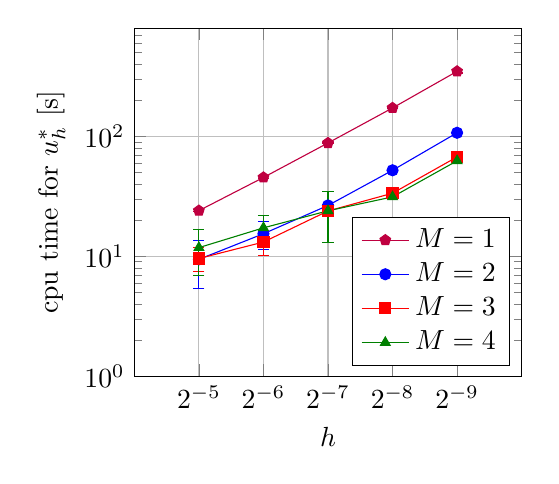
\begin{tikzpicture}
	\begin{semilogyaxis}[
		xlabel= {$h$},
		ylabel={cpu time for $u^*_h$ [s]},
		xmin = 0,
		xmax = 6,
		xtick = {1,2,3,4,5,6},
		xticklabels = {$2^{-5}$,$2^{-6}$,$2^{-7}$,$2^{-8}$,$2^{-9}$},%$2^{-10}$},
		ymin = 1,
		ymax = 800,
		%ytick = {0.001,0.01,0.1,1,10,100},
		xmajorgrids,
		ymajorgrids,
		width=6.5cm,
		height=6cm,
		legend pos=south east,
	]	
	
\addplot+ [purple, mark=pentagon*, mark options={purple},
error bars/.cd,y dir=both,y explicit,
] coordinates {
(1,24.0359) +- (0.4211,0.4211)
(2,45.4781) +- (0.9676,0.9676)
(3,88.1813) +- (1.3361,1.3361)
(4,172.8734) +- (2.1448,2.1448)
(5,349.4500) +- (10.7202,10.7202)
%(6,411.0859) +- (18.0826,18.0826)
};
\addlegendentry{$M = 1$};	
	
\addplot+ [blue, mark=*, mark options={blue},
error bars/.cd,y dir=both,y explicit,
] coordinates {
(1,9.4297) +- (4.0135,4.0135)
(2,15.4203) +- (4.0820,4.0820)
(3,26.5484) +- (0.3063,0.3063)
(4,52.1906) +- (1.2243,1.2243)
(5,107.2953) +- (1.4596,1.4596)
%(6,221.1094) +- (3.1966,3.1966)
};
\addlegendentry{$M = 2$};			
	
\addplot+ [red, mark=square*, mark options={red},
error bars/.cd,y dir=both,y explicit,
] coordinates {
(1,9.5844) +- (2.1702,2.1702)
(2,13.1438) +- (2.9098,2.9098)
(3,23.8875) +- (0.4702,0.4702)
(4,33.5969) +- (0.7035,0.7035)
(5,67.4875) +- (1.4545,1.4545)
%(6,174.5594) +- (18.2707,18.2707)
};
\addlegendentry{$M = 3$};	

\addplot+ [green!50!black,mark=triangle*, mark options={green!50!black},
error bars/.cd,y dir=both,y explicit
] coordinates {
(1,11.8109) +- (4.9417,4.9417)
(2,17.2703) +- (4.7307,4.7307)
(3,23.9641) +- (10.8673,10.8673)
(4,31.3062) +- (0.9268,0.9268)
(5,62.6500) +- (1.6013,1.6013)
%(6,154.6906) +- (3.2987,3.2987)
};
	\addlegendentry{$M = 4$};
	\end{semilogyaxis}
\end{tikzpicture}
\end{document}